\chapter{Abschätzung systematischer Fehler}
Der Fitter liefert uns zwar eine statistische Unsicherheit auf $\SJPsi$, allerdings ist eine Betrachtung der Systematik unerlässlich. Im Folgenden wird daher der Einfluss einiger Effekte auf das Fitergebnis untersucht und anschließend der systematische Fehler abgeschätzt.

\section{Fit Bias} \label{kap:fit_bias}
Die hier verwendete Maximum-Likelihood-Methode hat zwar den schönen Vorteil, dass das Fitergebnis nicht vom Binning abhängt, es ist jedoch nicht von vornherein ausgeschlossen, dass sie das Ergebnis verfälscht (einen sog. Bias produziert). Daher wird eine Toy Monte Carlo - Studie (kurz: Toy MC) durchgeführt. Dabei werden Daten zufällig nach einer Verteilung mit den gewünschten Parametern generiert und im Anschluss gefittet. Für eine gute Abschätzung des Bias dienen die Ergebnisse des Daten-Fits aus Tabelle xxxxxxx als Anhaltspunkt. Es werden pro Toy 20000 Teilchen generiert mit einem Signalanteil von 42,3\%.

\begin{figure}[hptb]
\centering
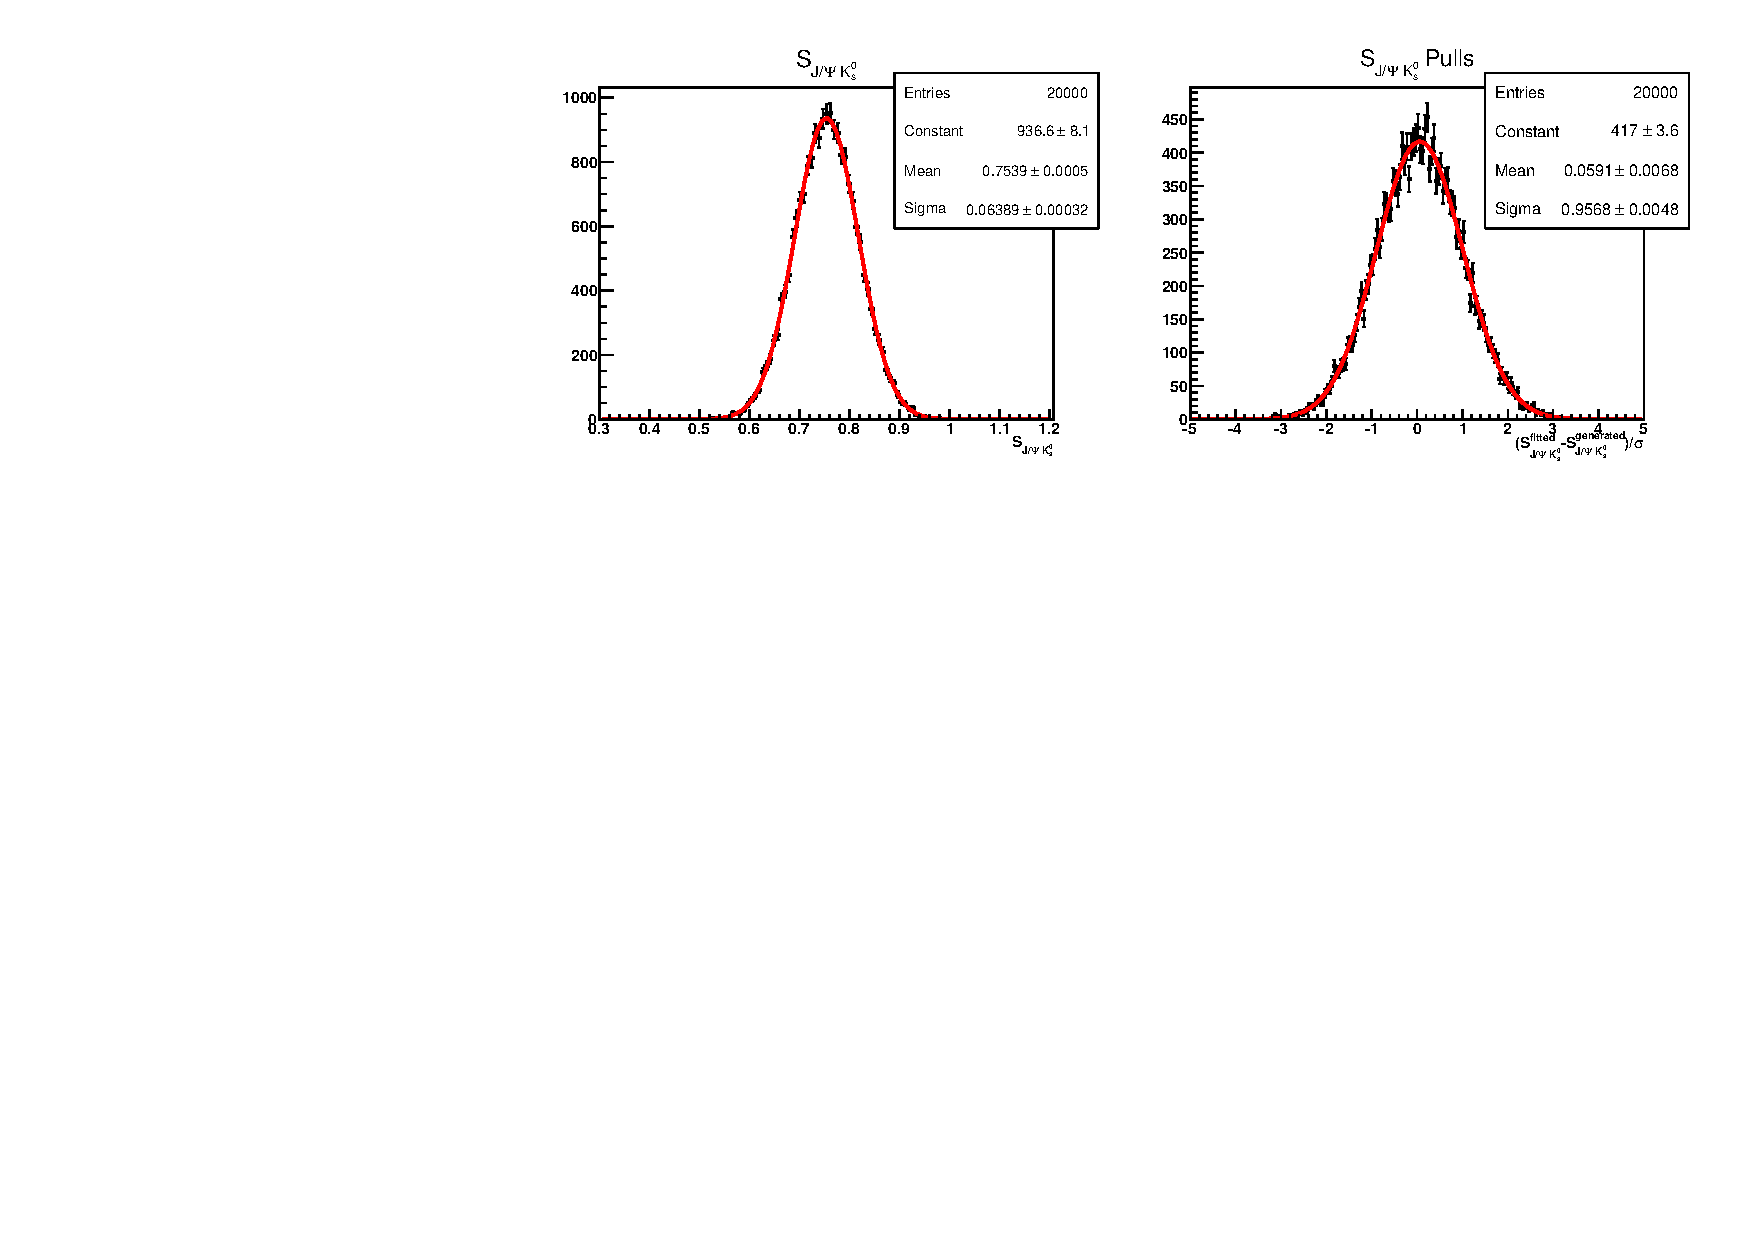
\includegraphics[width = \textwidth]{ampl_both}
\caption{Verteilung der aus der Toy MC Studie erhaltenen Amplituden $\SJPsi$ (links) sowie die dazugehörigen Pulls (rechts)}
\label{fig:fit_bias}
\end{figure}

Abbildung \ref{fig:fit_bias} zeigt sowohl die Verteilung der gefitteten Amplitude und die Pulls, die sich mittels $\frac{\SJPsi^{gefittet} - \SJPsi^{generiert}}{\sigma^{gefittet}}$ berechnen. Es lassen sich hierbei zwei Dinge beobachten:
\begin{enumerate}
    \item An der Verschiebung des Pull-Mittelwertes $\mu = 0,059 \pm 0,007$ von der Null sieht man deutlich, dass es einen kleinen, aber signifikanten Bias gibt. Indem wir diesen Bias mit der statistischen Unsicherheit aus unserem Fitergebnis (siehe Gl. \ref{eq:fit_result}) multiplizieren erhalten wir eine Abschätzung der aus der Fitmethode resultierenden Unsicherheit:
        \begin{align}
        \delta\SJPsi^{Fit} = 0,059 \cdot 0,07 = 0,00413
        \end{align}

    \item Mit einem $\sigma = 0,957 \pm 0,005$ ist die Pull-Verteilung signifikant zu schmal. Dies bedeutet, dass der Fit den statistischen Fehler überschätzt. Das Problem tritt auf, sobald man in den Toys Untergrund miteinbezieht. Es ist bekannt, dass die verwendete SFit-Methode die Fehlerpropagation (gerade bei Untergrund) nicht korrekt ausführt. Es wurde daher eine Fehlerkorrektur implementiert, aber auch dieser handelt es sich nur um eine Näherung.
\end{enumerate}

\paragraph{Ursachen des Bias}
Weitere Toy MC Studien zeigen, dass die Behandlung des Untergrundes zu einem Bias führt. Generiert man nämlich nur Signal, ist der Mittelwert kompatibel zur Null (siehe Abb. \ref{fig:toys_no_bkg}).

\begin{figure}[hptb]
\centering
%\includegraphics[width=\textwidth]{}
\caption{Toy MC Studie mit reinem Signal ohne Untergrund. Es kommt zu keinem signifikanten Bias. Links: Verteilung der erhaltenen Amplitude, Rechts: Pull-Verteilung.}
\label{fig:toys_no_bkg}
\end{figure}

Die Vermutung ist, dass zu wenig Statistik im Fit die eigentliche Ursache für den Bias ist. Daher wurden weitere Toy MC Studien mit unterschiedlicher Anzahl an Teilchen pro Toy durchgeführt. Die Ergebnisse sind in Tabelle \ref{tab:fit_bias_events} aufgeführt und in Abbildung \ref{fig:fit_bias_events} nochmals visualisiert.

\begin{table}[hptb]
\centering
\caption{Toy MC Studien mit unterschiedlicher Anzahl an generierten Events pro Toy. Genannt wird der Mittelwert $\mu$ der $\SJPsi$-Pull-Verteilung}
\label{tab:fit_bias_events}
\begin{tabular}{cr@{$\pm$}l}
\hline \hline 
Teilchen pro Toy & \multicolumn{2}{c}{$\mu$}  \\ \hline
20000            &  xxx & xxx \\
50000            &  xxx & xxx \\
100000           &  xxx & xxx \\
200000           &  xxx & xxx \\ 
\hline \hline
\end{tabular}
\end{table}

\begin{figure}[hptb]
\centering
%\includegraphics[width=\textwidth]{}
\caption{Visualisierung der Werte aus Tab. \ref{tab:fit_bias_events}}
\label{fig:fit_bias_events}
\end{figure}

\section{Tagging Kalibration}
Im Fit wird bei den Parametern der Tagging Kalibration nur der statistischen Fehler berücksichtigt. Es soll nun an dieser Stelle der Einfluss der statistischen Unsicherheiten abgeschätzt werden. \\
Die Korrekturparameter $p_0$ und $p_1$ für die Fehlerwahrscheinlichkeit des \gls{OST} sind gegeben durch
\begin{align}
p_0 &= 0,392 \pm 0,0017\ \text{(stat.)} \pm 0,0076\ \text{(syst.)} \\
p_1 &= 1,035 \pm 0,021\ \text{(stat.)} \pm 0,0076\ \text{(syst.)}.
\end{align}

\paragraph{Variation der Parameter in den Daten}
Zunächst werden die Startwerte der Parameter $p_0$ und $p_1$ variiert, indem man jeweils den systematischen Fehler der Parameter addiert bzw. subtrahiert und dann den Fit auf die Daten durchührt. Für alle vier Kombinationen wird dann die Abweichung vom regulären Fitergebnis für $\SJPsi$ berechnet. Der Referenzwert aus dem Fit beträgt
\begin{align}
\SJPsi = 0,625 \pm 0,069
\end{align}

\begin{table}[hptb]
\centering
\caption{Variation des Fitergebnisses für $\SJPsi$ bei Veränderung der Startwerte für $p_0$ und $p_1$ $\pm$ ihrer statistischen Unsicherheiten}
\label{tab:syst_fit_calib_data}
$\begin{array}{cc|c|c}
\hline\hline
p_0            & p_1           & \SJPsi          & \Delta\SJPsi   \\ \hline
0,392 - 0,0076 & 1,035 - 0,012 & 0,599 \pm 0,067 & -0,026 \pm xxx \\
0,392 + 0,0076 & 1,035 - 0,012 & 0,661 \pm 0,072 & 0,036 \pm xxx \\
0,392 - 0,0076 & 1,035 + 0,012 & 0,592 \pm 0,066 & -0,033 \pm xxx \\
0,392 + 0,0076 & 1,035 + 0,012 & 0,651 \pm 0,071 & 0,026 \pm xxx \\
\hline\hline
\end{array}$
\end{table}

Die Ergebnisse sind Tabelle \ref{tab:syst_fit_calib_data} zu entnehmen. Die größte Abweichung beträgt hier $\Delta\SJPsi = 0,036$.

\paragraph{Variation der Parameter in \gls{Toy MC}}
Eine weitere Möglichkeit der Abschätzung besteht darin, sich entsprechende Toys zu generieren und diese dann zu fitten. Im Folgenden werden bei der Toy Generierung die Parameter $p_0$ und $p_1$ um ihre systematische Unsicherheiten variiert, der Fit dann allerdings mit den ursprünglichen Parameterwerten durchgeführt. Als Referenzwert generieren und fitten wir toys mit den ursprünglichen Parameterwerten $p_0$ und $p_1$ sowie $\SJPsi = 0.75$ und erhalten hierfür:

\begin{align}
\SJPsi = 0,75527 \pm xxx
\end{align}

\begin{table}[hptb]
\centering
\caption{Variation des Fitergebnisses für $\SJPsi$ bei Veränderung der Parameterwerte $p_0$ und $p_1$ $\pm$ ihrer statistischen Unsicherheiten bei der Generierung von Toys}
\label{tab:syst_fit_calib_toys}
$\begin{array}{cc|c|c}
\hline\hline
p_0            & p_1           & \SJPsi          & \Delta\SJPsi   \\ \hline
0,392 - 0,0076 & 1,035 - 0,012 & 0,782 \pm xxx & 0,027 \pm xxx \\
0,392 + 0,0076 & 1,035 - 0,012 & 0,719 \pm xxx & -0,036 \pm xxx \\
0,392 - 0,0076 & 1,035 + 0,012 & 0,788 \pm xxx & 0,032 \pm xxx \\
0,392 + 0,0076 & 1,035 + 0,012 & 0,727 \pm xxx & -0,028 \pm xxx \\
\hline\hline
\end{array}$
\end{table}

Die Ergebnisse sind Tabelle \ref{tab:syst_fit_calib_toys} zu entnehmen. Die größte Abweichung beträgt hier betragsmäßig ebenfalls $\Delta\SJPsi = 0,036$. Daher schätzen wir den systematischen Fehler durch die Tagging Kalibrierung auf 

\begin{align}
s_{tag_calib} = 0.036 \ .
\end{align}

\section{Einfluss der zeitlichen Akzeptanz}
In der Analyse wurde der Einfluss einer zeitabhängigen Detektorakzeptanz vernachlässigt. Nimmt man an, dass sich die Akzeptanz von \Bd- und \Bdbar-Mesonen nicht unterscheiden, so hat die Akzeptanz keinen Einfluss auf die Asymmetrie, da sie sich hier herauskürzt. Beim Fit der Amplitude nach Gleichung \ref{eq:fit_pdf} ist dies aber nicht zwangsläufig so. Um hiesiges Vorgehen zu rechtfertigen, wird zunächst eine Bestimmung der Akzeptanz durchgeführt und anschließend mit einer Toy MC Studie ihr Einfluss überprüft.

\subsection{Bestimmung einer Akzeptanzfunktion} \label{kap:akzeptanz_bestimmung}
\Bd-Mesonen haben eine relativ lange Lebensdauer. Um sie von kurzlebigem Untergrund zu unterscheiden, befinden sich auf den Triggern und dem Stripping entsprechende Cuts auf die Flugzeiten. Dies hat zur Folge, dass für kleine Flugzeiten ($ct \lesssim 0,3\pico\second$) kaum \Bd-Mesonen im Detektor registriert werden und es zu einem sog. \glqq Turn-On-Effekt\grqq kommt. Es hat sich herausgestellt (\cite{lhcb-paper}), dass dieser gut durch die Funktion
\begin{align}
\epsilon_1(t) = \frac{2}{\pi}\arctan[t\cdot \exp(at+b)]
\end{align}
parametrisiert wird.

Je länger ein \Bd-Meson lebt, desto schwieriger wird es, die Zerfallsprodukte im Detektor auf Grund seiner begrenzten Länge nachzuweisen. Daher nimmt die Akzeptanz zu großen Zeiten hin wieder ab. Zur Parametrisierung fällt die Wahl auf eine lineare Funktion
\begin{align}
\epsilon_2(t) = 1 + \beta t \qquad (\beta < 0).
\end{align}

Die entsprechende gesamte Akzeptanzfunktion lautet demnach:
\begin{align}
\epsilon(t) = \epsilon_1(t) \cdot \epsilon_2(t) = \frac{2}{\pi}\arctan[t\cdot \exp(at+b)](1 + \beta t)
\end{align}

Zur Bestimmung der Paramater wird die Trennung von \Bd- und \Bdbar-Mesonen aufgehoben, sodass lediglich ein exponentieller Zerfall zu beobachten ist. Des weiteren wird der Cut auf die Lebensdauer bei $0,3\pico\second$ nicht angewandt, sodass der Turn-On-Effekt auch richtig sichtbar wird. Die Wahrscheinlichkeitsdichtefunktion für den Fit lautet somit:
\begin{align}
\mathcal{P}_{acc}(t) \propto \epsilon(t)\cdot \e^{-t/\tau} = \e^{-t/\tau}\cdot\frac{2}{\pi}\arctan[t\cdot \exp(at+b)](1 + \beta t)
\end{align}

Die beiden Parameter $\tau$ und $\beta$ sind stark miteinander korreliert. Für eine geeignete Bestimmung der Parameter der Akzeptanz-Funktion wird daher die Lebensdauer auf den PDG-Wert $\tau = 1,519 \pm 0,007 \pico\second$ \cite{pdg-tau} constraint, die anderen Parameter fließen. Die Ergebnisse sind in Tabelle \ref{tab:fit_akzeptanz} aufgeführt, die entsprechenden Plots in Abbildung \ref{fig:fit_akzeptanz}. 

\begin{table}[hptb]
\centering
\caption{Ergebnis des Fits zur Bestimmung der zeitlichen Akzeptanz}
\label{tab:fit_akzeptanz}
\begin{tabular}{lr@{$\pm$}l}
\hline \hline 
Parameter & \multicolumn{2}{c}{Ergebnis}  \\ \hline
$\tau$    &  1,519   & 0,007 \\
$a$       &  44,1    & 5,7 \\
$b$       &  -7,4    & 1,1 \\
$\beta$   &  -0,0056 & 0,0085 \\ 
\hline \hline
\end{tabular}
\end{table}

\begin{figure}[hptb]
\centering
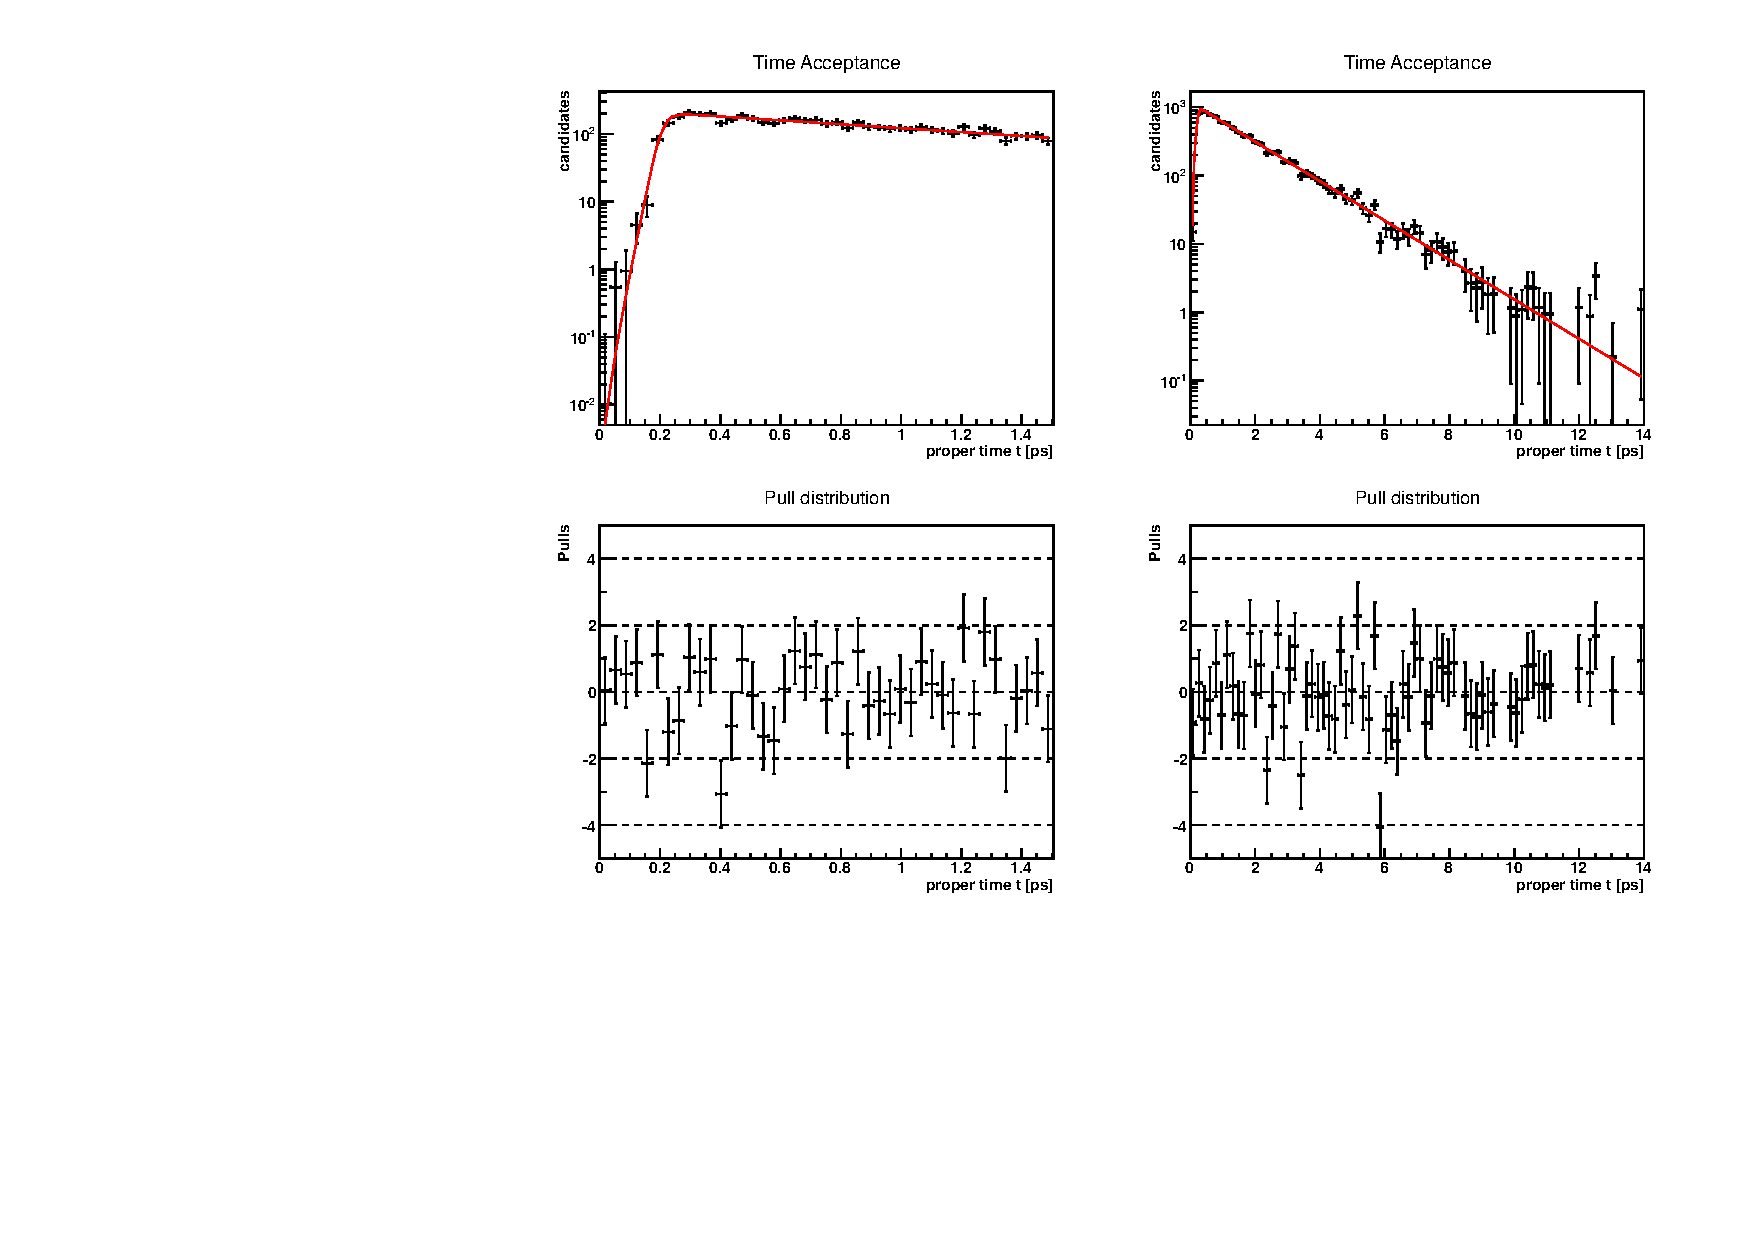
\includegraphics[width=\textwidth]{time_acceptance_fit}
\caption{Fit an die Flugzeit-Verteilung aller \Bd-Mesonen mit eingeschlossener Akzeptanzfunktion (oben) sowie die entsprechende Pull-Verteilung (unten). Links: kurzlebiger Zeitbereich ($t<1,5\pico\second$), Rechts: gesamtes Flugzeitspektrum ($0\ps < t < 14\ps$)}
\label{fig:fit_akzeptanz}
\end{figure}

\subsection{Bestimmung des Einflusses}
Durch den Cut auf die Lebensdauer bei $t = 0,3\ps$ in der Datenselektion spielt der Turn-On-Effekt im hier verwendeten Datensatz eigentlich keine Rolle. Dies wird dadurch deutlich, dass die Akzeptanzfunktion $\epsilon(0,3\ps) = 0,992$ und damit fast Eins ist. Auch am Ende des Analysebereichs beträgt die Akzeptanz noch $\epsilon(14\ps) = 0,905$. Daher liegt die Vermutung nahe, dass sich die Akzeptanz nicht gravierend auf das Fitergebnis auswirkt. Mit den in Kapitel \ref{kap:akzeptanz_bestimmung} bestimmten Parametern wird die zeitliche Akzeptanz bei der Erzeugung der Toys berücksichtigt, der anschließende Fit aber ohne Akzeptanzfunktion durchgeführt. Die zur Erzeugung verwendeten Parameter entsprechen ansonsten denen in Kapitel \ref{kap:fit_bias}.

\begin{figure}[hptb]
\centering
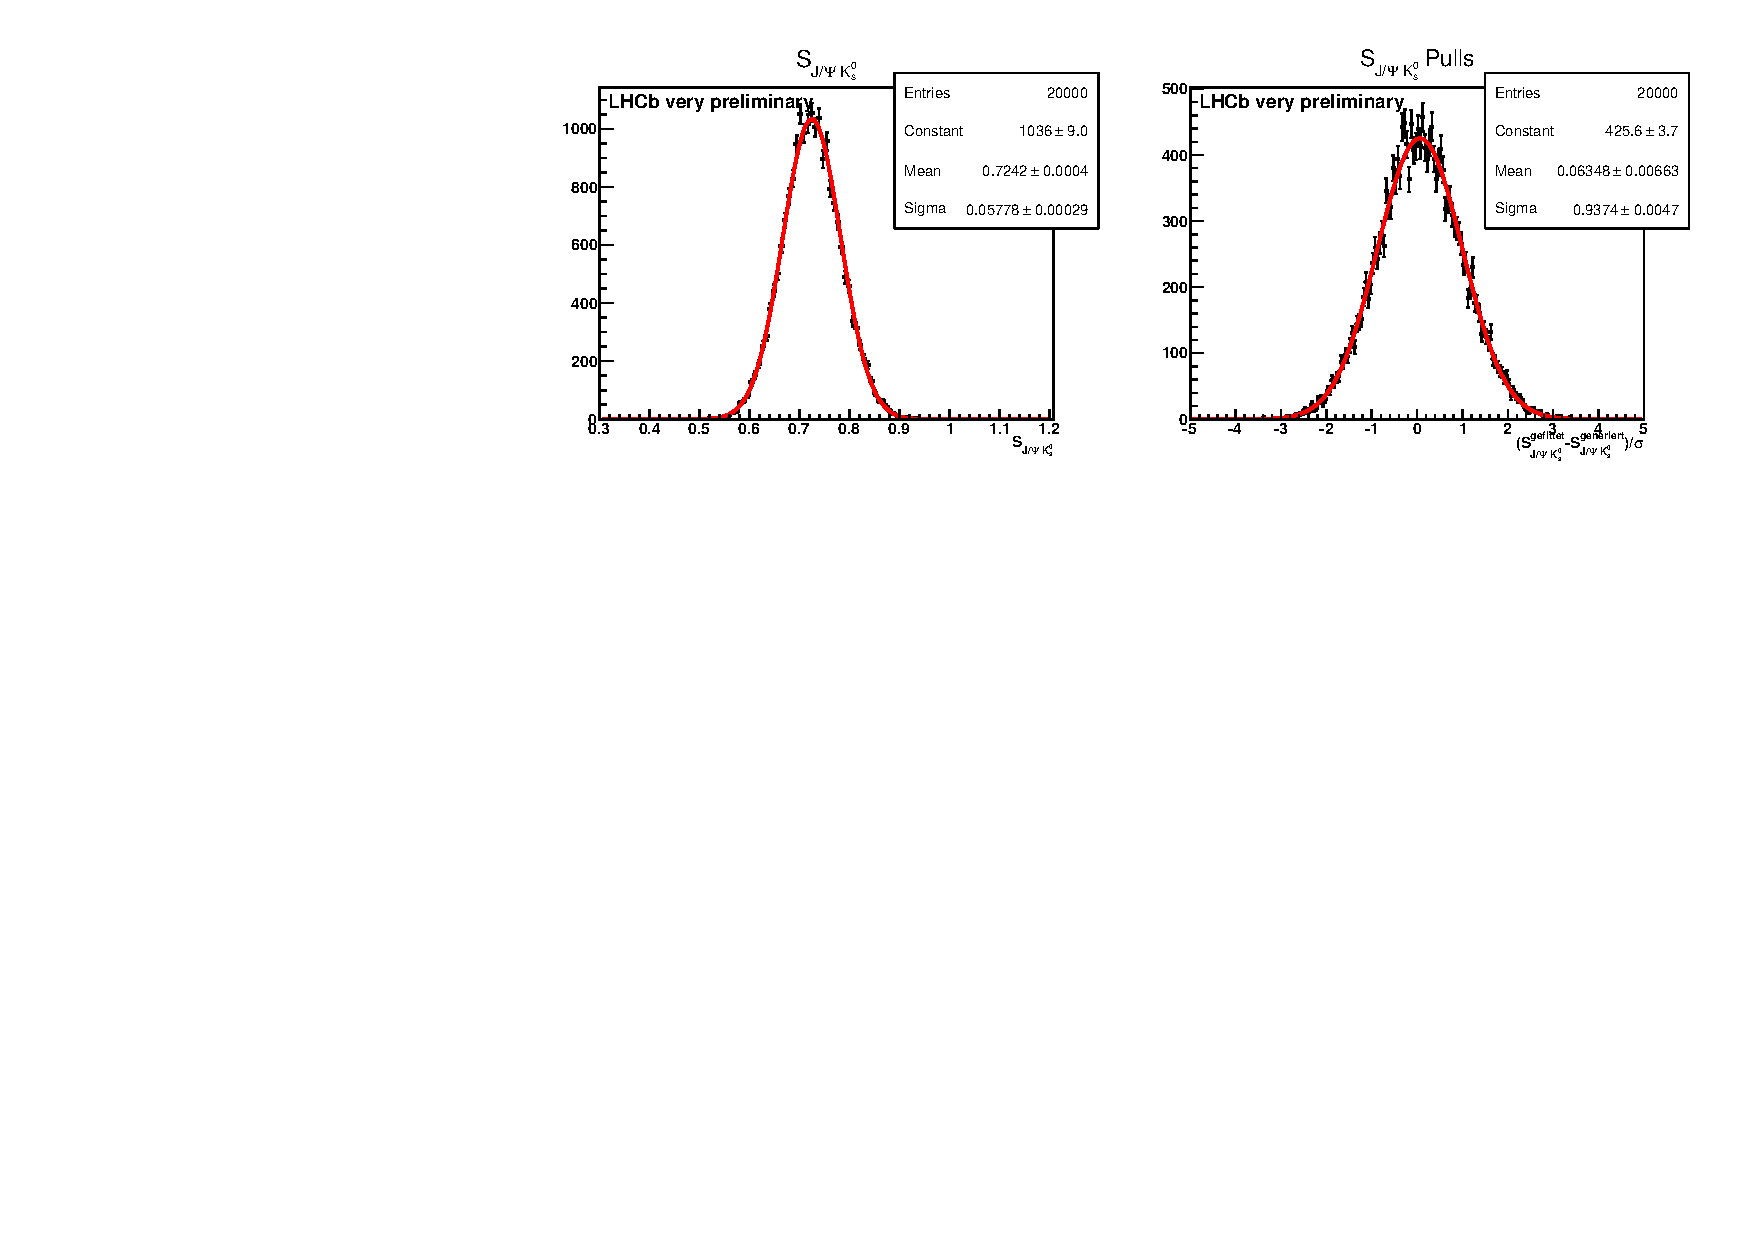
\includegraphics[width = \textwidth]{time_acceptance_toys}
\caption{Untersuchung des Einflusses einer zeitlichen Akzeptanz: Verteilung der aus der Toy MC Studie erhaltenen Amplituden $\SJPsi$ (links) sowie die dazugehörigen Pulls (rechts)}
\label{fig:toys_acceptance}
\end{figure}

Der Mittelwert der Pulls $\mu = 0,063 \pm 0,007$ (siehe Abb. \ref{fig:toys_acceptance}) ist kompatibel mit dem aus dem Fit Bias erhaltenen $\mu = 0,059 \pm 0,007$ und erzeugt dementsprechend keinen signifikanten zusätzlichen Bias. Damit ist die Vernachlässigung der zeitlichen Akzeptanz im Fit gerechtfertigt.



\section{Gleichförmigkeit der Massenverteilung}
